\section{Ausblick}

    Neue Entwicklungsziele und Konzepte im Bereich des teil- und vollautonomen Fahrens stellen die elektronischen Fahrzeugsysteme vor Herausforderungen, die mit den heute
    verwendeten Systemen noch nicht bewältigt werden können.\\
    Die selbstständige Durchführung der Fahraufgabe durch ein elektronisches System oder die aktive Unterstützung eines menschlichen Fahrzeugführers
    bedingt eine umfangreiche Erfassung und Auswertung sämtlicher Fahrzeug- und Umgebungsdaten.\\
    Zu diesem Zweck müssen die klassischen Sensorsysteme um neue Systeme erweitert werden, die zum Beispiel optische Umweltdaten über Kameras liefern, Umgebungsscans
    mittels Radar, Lidar oder Ultraschall durchführen und die in der Lage sind, diese Daten in Echtzeit auszuwerten und zu verarbeiten. ~\cite{BP06}\\

    Während insbesondere zu Beginn der Entwicklungs- und Integrationsphase die Fahrzeuge noch autarke Einheiten sind, die alle für die
    Fahraufgabe notwendigen Daten eigenständig erheben müssen ist das langfristige Hauptziel von Industrie und Rechtsgebern eine umfassende Vernetzung
    sämtlicher Entitäten, die am Verkehrsgeschehen aktiv oder passiv partizipieren zu einem intelligenten Transportation System (ITS).\\

    Ein solches ITS soll den Teilnehmern innovative Dienste anbieten, mit dem Ziel das Verkehrsgeschehen
    effizient zu verwalten und zu koordinieren, die Umwelteinwirkungen durch Kraftfahrzeuge zu senken und erhöhte Sicherheit für alle 
    aktiv und passiv am Verkehrgeschehen beteiligten zu bieten. ~\cite{BP04} \cite{BP11}\\

    Denkbare Szenarien sind zum Beispiel der aktive Austausch von Geschwindigkeits- und Richtungsdaten von Fahrzeugen in der näheren Umggebung, um unnötige Brems-
    und Beschleunigungsvorgänge zu vermeiden, sowie die Übertragung auslastungsspezifischer Geschwindigkeitsbegrenzungen von smarten Verkehrsschildern
    direkt an die Fahrzeuge. Auch eine kontaktlose Erfassung und Verrechnung von nutzungsabhängigen Straßengebühren wäre denkbar und ist bereits im Einsatz.\\

    Dies sind nur einige Beispiele der Möglichkeiten eines voll vernetzten Transportsystems, das umfangreiche Datenerfassung mit Ad-Hoc Kommunikationsmöglichkeiten und
    modernen Prognose- und Analysealgorithmen vereint.

    Das Konzept eines solchen ITS bedingt jedoch, dass alle Teilnehmer als unabhängige Knoten in der Lage sind, miteinander zu kommunizieren.

    Die Vernetzung zweier Knoten in einem ITS kann anhand der Art der Knoten, die miteinander kommunizieren, kategorisiert werden.

    \subsection{Vehicle to Everyhing}
    Grundlage eines ITS ist die \textbf{Vehicle to Everything} Kommunikation, die das Fahrzeug als zentralen Punkt in den
    Kontext der unterschiedlichen Umgebungssysteme und Entitäten setzt. Dabei wird genauer unterschieden in die Teilbereiche:
    
    \subsubsection{Vehicle to Vehicle}
    \textbf{Vehicle to Vehicle} (V2V) beschreibt die Ad-Hoc Vernetzung mehrerer Fahrzeuge untereinander mit dem Ziel relevante Fahrzeugdaten z.Bsp. über Richtung und Geschwindigkeit auszutauschen.
    Desweiteren sollen über V2V Kommunikation weitere sicherheitsrelevante Nachrichten aus anderen Teilbereichen weitergeleitet werden.

    \subsubsection{Vehicle to Network}
    \textbf{Vehicle to Network} (V2N) beschreibt die Vernetzung des Fahrzeugs mit dem Telekommunikationsnetz und der Cloud. Dadurch können über den
    rein lokalen Kontext hinaus Ressourcen genutzt und Daten geteilt werden. Ein Beispiel für eine solche V2N Anwendung, die bereits heute
    im Einsatz ist, ist die Integration cloudbasierter Navigationslösungen wie Google Maps in das Fahrzeug.
    
    \subsubsection{Vehicle to Infrastructure}
    \textbf{Vehicle to Infrastructure} (V2I) (alternative Bezeichnung: Vehicle to Roadside) beschreibt die Vernetzung des Fahrzeugs mit der umgebenden Verkehrsinfrastruktur. 
    Zum Beispiel könnten Mautstationen automatisiert Fahrzeuge erfassen und abrechnen oder smarte Ampelanlagen könnten die Ampelzyklen in Abhängigkeit
    der Anzahl der jeweils wartenden Fahrzeuge anpassen, um den Verkehrsfluss zu optimieren. 

    \subsubsection{Vehicle to Pedestrian}
    \textbf{Vehicle to Pedestrian} (V2P) beschreibt die Vernetzung des Fahrzeugs mit nichtmotorisierten Verkehrsteilnehmern.
    Während bei den restlichen Vernetzungarten beide Endknoten als elektronische Systeme definitionsgemäß vernetzungsfähig sind, ist bidirektionale V2P Kommunikation nur möglich
    falls der nichtmotorisierte Verkehrsteilnehmer ein entsprechendes Gerät, zum Beispiel ein Smartphone mitführt, dass diese Funktionalität unterstützt.
    Daher ist V2P ist auch allgemeiner zu verstehen und umfasst neben der aktiven bidirektionalen Kommunikation der Entitäten auch die Erfassung von Fussgängern über rein
    fahrzeugseitige Sensorsysteme.

    Ziel von V2P ist explizit der Schutz der nichtmotorisierten Verkehrsteilnehmer, die bei Unfällen einen inhärenten Nachteil haben.

    \subsubsection{Vehicle to Device}
    \textbf{Vehicle to Device} (V2D) beschreibt die Kommunikation des Fahrzeugs mit elektronischen (Hand-)Geräten. Aktuelle Einsatzgebiete für diese Form der Kommunikation
    sind mobile Applikationen für Smartphones, mit denen Fahrzeugfunktionen von außerhalb gesteuert werden können. Beispiele hierzu
    sind die Smartphone Applikation von Tesla, mit der Fahrzeuge ausgeparkt werden können oder eine neue Entwicklung von Volvo mit der physische Schlüsseltechnologie
    durch eine mobile Smartphoneapp zuerst ergänzt und später ersetzt werden soll. ~\cite{BP05}
     
    \subsubsection{Vehicle to Grid}
    \textbf{Vehicle to Grid} (V2G) beschreibt die Vernetzung eines elektrischen Fahrzeuges mit dem Stromnetz mit dem Ziel die Batterien elektrischer Fahrzeuge als Speichermedien
    bidirektional in das Stromnetz zu integrieren. \cite{BP08}

    \subsection{ITS Technologie und Standardisierung}

    Aufgrund der heterogenen Landschaft an Fahrzeugherstellern, Infrastrukturbetreibern, Komponententechnologien und der Tatsache, dass Möglichkeiten
    und Beschränkungen dieser neuartigen Technologien noch nicht ausgelotet sind wurde bereits früh ein konkreter Standardisierungs- und Normierungsbedarf erkannt.

    Aus dieser Erkenntnis heraus sind die wichtigsten Standardisierungsorganisationen ISO, CEN, ETSI und SAE dabei Referenzarchitekturen und Protokolle zu entwickeln, die
    die Grundlagen der Weiterentwicklung der Technologie in die Zukunft bilden sollen.\cite{BP11}\\
    Da die Lebens- und Nutzungsspanne von Fahrzeugen mittlerweile bei 15 Jahren angelangt ist und in naher Zukunft bis zu 20 Jahren prognostiziert werden, während gleichzeitig die 
    Lebensspanne von Kommunikationsmedien immer kürzer wird liegt die grundlegende Schwierigkeit der Standardisierungsbemühungen darin, zukunftssichere Standards und Protkolle zu entwickeln,
    die von konkret verwendeten Kommunikationsmedien abstrahieren und sicherstellen, dass Fahrzeuge, die heute produziert werden auch in 20 Jahren noch ohne nennenswerte Einbussen der Funktionalität in die Verkehrssysteme
    integriert werden können. Da es für die Hersteller zudem nicht kosteneffizient ist, Fahrzeuge für regionale Märkte zu produzieren, müssen die Lösungen für ITS Systeme
    außerdem globale Einsatzmöglichkeiten bieten.\\
    Mit diesem Ziel hat die ISO mit der ISO 21217 \cite{BP09} bereits im Jahr 2010 die CALM Referenzarchitektur konkretisiert, die eine schichtbasierte Lösung präsentiert, die die Applikationsschicht, in
    der die intelligenten Transportsysysteme ihre Dienste bereitstellen und nutzen von der medienbasierten Kommunikation trennt.\\
    Die CALM Architektur bildet die Grundlage aller internationalen Standardisierungsbemühungen.

       
    \begin{figure}[h!]
        \begin{center}
        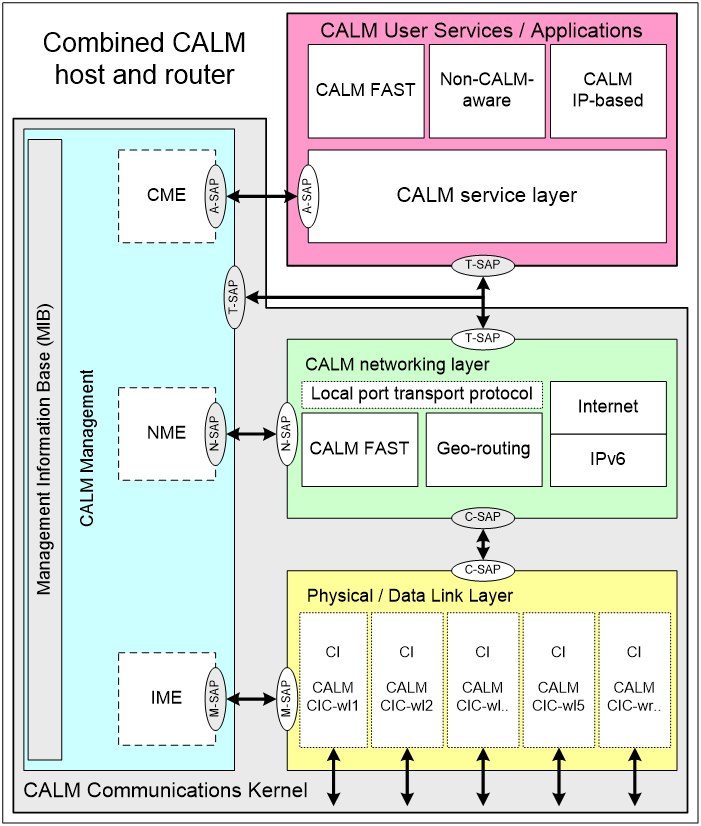
\includegraphics[width=0.7\linewidth]{./images/BP/CALM.png}
        \caption[]{CALM Architektur \cite{BP07}}
        \label{fig:CALM}
    \end{center}
    \end{figure}

    Aufbauend auf dieser Referenzarchitektur existieren spezifische Konkretisierungen für die verschiedensten drahtlosen und drahtgebundenen Kommunikationsmedien.
    Die zwei wichtigsten Spezifikationen sind dabei die drahtlose Kommunikation auf der Grundlage von WLAN, die aufbauend auf der IEEE 802.11a Spezifikation im IEEE 802.11p Protokoll \cite{BP10} spezifiert ist 
    und das 3GPP Protokoll für eine drahtlose Kommunikation auf Basis von Mobilfunktechnologie.

    \subsubsection{IEEE 802.11p}
    Der IEEE 802.11p Standard, spezifiziert eine Erweiterung des IEEE 802.11 WLAN Standards, der die drahtlose Kommunikation in und mit Fahrzeugen ermöglicht.

    Diese Erweiterung war notwendig, da die Zeitspanne zur Kommunikation eines Fahrzeugs in Bewegung mit stationären Infrastrukturknoten meist nur sehr kurz ist, was prohibitiv für die komplexe Verbindungsaufbauphase
    im herkömmlichen WLAN ist. Daher ermöglicht 802.11p die sofortige Kommunikation der Teilnehmer, ohne zuvor ein Basic Service Set zu etablieren.\\
    Da dies jedoch bedeutet dass die kommunizierenden Stationen nicht assoziert und nicht authentifiziert sind, müssen entsprechende Sicherheitsmechanismen in höheren Netzwerkschichten
    implementiert werden.

    IEEE 802.11p bildet den Grundstein für die Dedicated Short Range Communication Technik (DSRC), die in Europa als ITS-G5 bezeichnet wird. 
    
    Neben der drahtlosen Kommunikation auf Grundlage von WLAN, ist besonders für die Vernetzung über längere Entfernung die Verwendung bestehender oder zukünftiger Mobilfunksysteme möglich.
    Diese Kommunikationstechnologien werden in der 3GPP Protokollfamilie spezifiziert.

   
    \subsection{Zusammenfassung und Fazit}
    Die Einbindung immer komplexerer elektronischer Systeme in Fahrzeugen hat die Entwicklung in den vergangenen
    20 Jahren rasant vorangetrieben. Zum Teil veraltete Standards müssen überdacht und modernisiert werden.\\
    Entwicklungen in der nahen Zukunft, die das Fahrzeug aus dem individuellen Kontext herauslösen und in ein holistisches volllvernetztes
    System integrieren mit dem Ziel erhöhter Sicherheit, verminderter Auswirkungen der Mobilität auf die Umwelt und der Entwicklung neuer Geschäftsmodelle
    und Mobilitätskonzepte stellen eine Herausforderung an die Standardisierungsorganisationen, da die Zusammenführung und Kooperation heterogener Systeme zu einem
    vereinheitlichten Gesamtsystem nur auf Grundlage zukunftsfähiger Standards möglich ist.\\
    
    Zudem bedeuten neue Antriebskonzepte wie Hybridmotoren oder rein elektrische Antriebe, dass sich die Landschaft elektronischer Fahrzeugsysteme bereits kurzfristig 
    weiter verändern wird. Viele Sensorsysteme zur Überwachung der mechanischen Motorkomponenten werden in elektrisch betriebenen Fahrzeugen obsolet, während
    neue komplexe Sensorsysteme, die teil- und vollautonomes Fahren ermöglichen, zunehmend Einzug in die Fahrzeuge halten werden.\\

    Daher kann und soll diese Ausarbeitung nur ein Ausgangspunkt für eine weitere Erschliessung des Themas in der gesamten Komplexität darstellen.
